\section{Ensemble}
A number of different strategies for combining the ensemble members will be described in this section. This includes averaging and weighted averaging the detections. The method for inferring each of the ensemble will be the same apart from the combination set. This is shown in \figref{ensemble_general}. Firstly, for a object proposal in an image found with the \gls{rpn} each network will infer a bounding box and associated confidence for all classes. After this the given ensemble combination method determines the final detection. 
\begin{figure}[H]
  \centering
    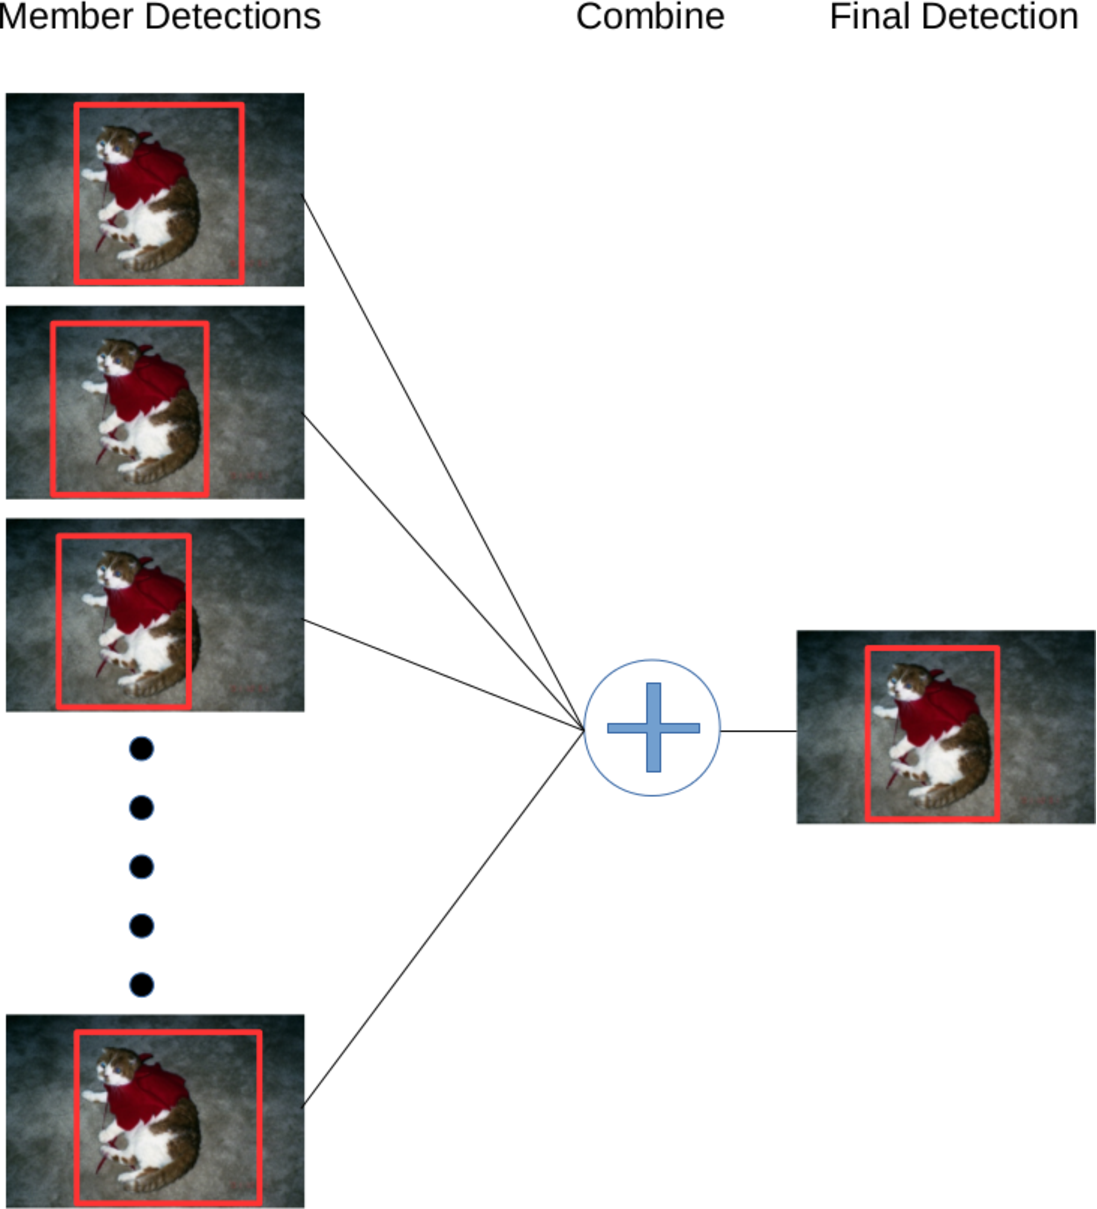
\includegraphics[width=0.5\textwidth]{Figs/Implementation/ensemble.pdf}
      \caption{}
    \label{fig:ensemble_general}
\end{figure}

A number of different combination strategies will be presented and evaluated in the remainder of this section. 

\subsection{Average Ensemble}
One of the combination strategies is similar to that used when evaluating the resolution-aware object detector in \sectionref{resawareSec}. Each of the five ensemble factors are weighted evenly in the overall ensemble. Within each ensemble factor pair, the detection for one of the pairs will be chosen and the other discarded. This is determined by where the given factor lies in relation to the training data distribution. For example, if for the given test image it is measured with Deep IQA to have JPEG compression below the threshold used to split the data, then the detection found using the model trained on that data will be used. This results in five detections that will be weighted equally to find the final detection by:

\begin{equation}
  E_{j} = \frac{1}{n} \sum_{i=1}^{n} p_{i,j} 
\end{equation}
where $n$ is the number of detections found by the $n$ ensemble factor, $p$ is the detection result to be averaged and $i$ represents one of the ensemble factors. Finally, $j$ is one of the five values found by each detection, namely the four corners of the bounding-box and the associated confidence.


\subsection{Weighted Average Ensemble}
Each of then 10 trained networks will be used on all object proposals found using the \gls{rpn}. Weights will be distributed evenly across each of the five different types of factors. The weighted average ensemble is determined for each bounding-box and the associated confidence by:

\begin{equation}
	E_{j} = \frac{1}{n} \sum_{i=1}^{n} w_ip_{i,j} 
\end{equation}

Weights are determined in pairs for each of the 5 ensemble factors, where the total sum of weights is equal to $n$. If each detection were to be weighted equally all $w$ would be equal to 1. As the weights are calculated in pairs each ensemble factor is overall weighted equally as the pair of weights can at most be equal to 2. By using this tactic in between the two sets of network for a given factor can be weighted differently but overall each factor is weighted equally.
Weights for a given factor is found according to where the the test image lies for that factors training distribution data. For example, the subsets of training data for Gaussian blur was determined according to the line shown in \figref{blur_dist}. 

\add[inline]{line showing split in training data}

\begin{figure}[H]
  \centering
    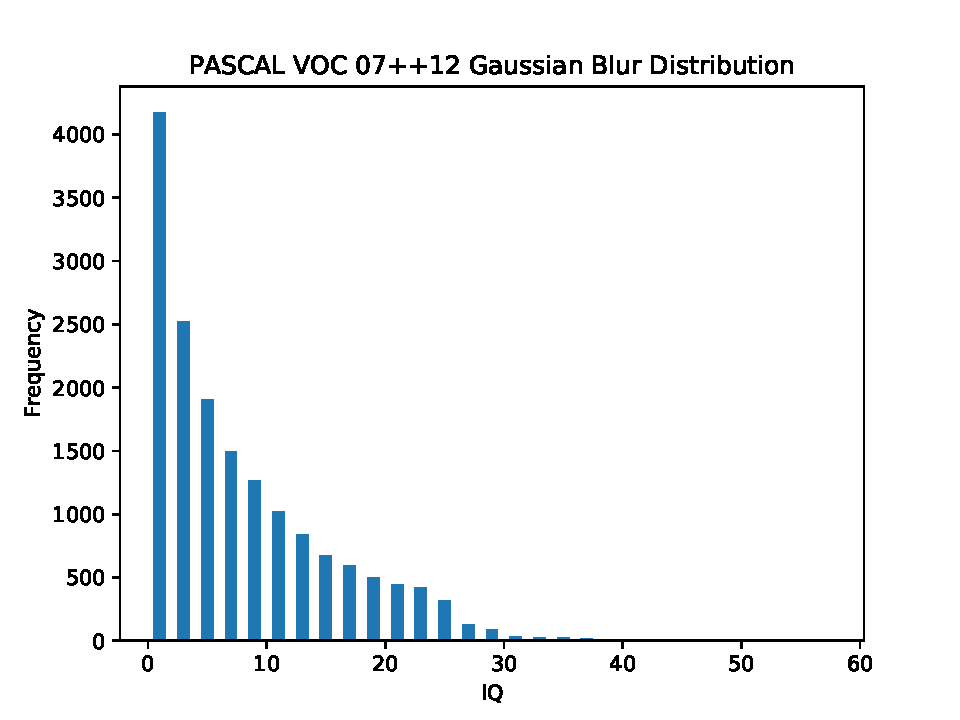
\includegraphics[width=0.8\textwidth]{Figs/Implementation/GaussianBlurdist.pdf}
      \caption{}
    \label{fig:blur_dist}
\end{figure}

The quality, $q_i$ with respect to blur for a given image is determined using the appropriate Deep IQA model, if the quality is below the value used to split the data the weights are calculated for the detection found with the given lower network by:

\begin{equation}
	w_{Lower} = 2 - \frac{split - q_i}{split - minq_i}
\end{equation}

and the weight for the upper network $w_{Upper}$ by:

\begin{equation}
	w_{Upper} = 2 - w_{Lower}
\end{equation}

where $split$ is the value used to split the training data and $minq_i$ is the minimum quality for the given factor in the training set.

However, if the quality is above $split$ the $w_{Upper}$ is calculated by:

\begin{equation}
	w_{Upper} = 2 - \frac{maxq_i - q_i}{maxq_i - split}
\end{equation}

and lower weight $w_{Lower}$:

\begin{equation}
	w_{Lower} = 2 - w_{Upper}.
\end{equation}

\subsubsection{Results}
In this section the results for the two above mentioned ensemble combinations strategies will be presented. Each presentation will be accompanied with the result for the baseline R-FCN ResNet-101 model trained on all of the 07++12 training data and will be dubbed as baseline. The results presented will be on the 2007 \gls{pascalvoc} test set as also shown in earlier preliminary results in this report.
\\\\
The results for both combination strategies can be seen in \tableref{avgres1}.

\begin{table}[h]
\centering
\caption{Results for the two ensemble combination strategies and for the baseline model on the 2007 test set.}
\label{tab:avgres1}
\begin{tabular}{|l|l|}
\hline
\textbf{Method}           & \textbf{AP (\%)} \\ \hline
Average          & 79.21\% \\ \hline
Weighted Average & 79.13\% \\ \hline
Baseline         & \textbf{79.59\%} \\ \hline
\end{tabular}
\end{table}

While neither of the combinations provide an improvement over the baseline method both provide an increase in performance in comparison to the image quality expert results found shown in \sectionref{iq_experts} 


